\documentclass[11pt,a4paper,twocolumn]{article}
\usepackage{paper}

\author{Clifford Chou, Favian Contreras, Bryan Cuccioli, Lee Gao}
\title{Scale-Free Networks in Static Call Graphs}
\date{\today}

% Prevent inline equations from breaking across lines
\relpenalty=10000
\binoppenalty=10000

% We only want this in the final report, not the intermedidate report.
\setlength{\jot}{.3cm}
\makeatletter
\renewcommand*\env@matrix[1][\arraystretch]{%
  \edef\arraystretch{#1}%
  \hskip -\arraycolsep
  \let\@ifnextchar\new@ifnextchar
  \array{*\c@MaxMatrixCols c}}
\makeatother

\begin{document}
\begin{singlespace}
\twocolumn[
  \begin{@twocolumnfalse}
    \maketitle
    \begin{abstract}
{We explore a novel approximate measure of the efficiency of large-scale
software engineering projects. Many software systems are so large and complex
that it is impossible to reason about their runtime properties using
conventional techniques in runtime analysis. Our approach treats the
interaction between the different subroutines of a system as network behavior
and approximates the running time via the distribution of static function
calls.}

{Having experimentally determined that various large software systems
behave like scale-free networks, we gain an asymptotic characterization of the
growth of the max-degree node within the call-graph, which lets us approximate
 the running time of such systems with code size $n$ according
to $O\left(\sqrt[\alpha]{n}\right)$ for $\alpha \approx 1.23$.}
    \end{abstract}
    \hspace*{7,6mm}\textit{Keywords:} {\sf \small scale-free networks, software
engineering, static analysis, linear interpolation}

\vspace{10pt}
  \end{@twocolumnfalse}
]


\section{Introduction}

A big problem in software engineering is attempting to reason about
the efficiency of the software system being developed. Traditional runtime
analysis techniques tend to focus on algorithms as individual components.
Because of the inherent difficulty in exploring the relationship between
large numbers of different components of the system, such techniques are
rarely amenable to large-scale projects.

Traditional techniques are rather cumbersome to wield and require a lot of
sophisticated machinery and analysis.
Oftentimes, these techniques do not scale to large
projects with complex caller-callee relationships between their various subroutines.
However, conventional wisdom and anecdotal experience in the profiling and
optimization of software code indicate
that most of the benefits come from reducing the complexity of
the functions that get called most often. As such, we devise a measure of the
complexity of a project based on how many incoming function calls each
function might receive.

Using this rule of thumb, one might then view the complexity of the caller-callee
relationship of each function as a statistical measure of the the runtime of the
software been developed. For example, if a subroutine $f$ is called by a million
different functions, then by reducing the overall runtime of $f$ by a small factor
might net us a million-fold increase in efficiency. Indeed, it has been observed
time and time again \cite{BENCH} that the most-called function of a program
is typically the bottleneck in the software runtime. Therefore, a natural idea for
measuring the complexity and the bloat of a large software project is to measure
the expected \emph{most} number of calls that any function within the software
will receive.

While this expected maximum number of called function is somewhat difficult and
tedious to compute, we found that it is possible to accurately
estimate this statistic using only the number of functions alone. We introduce a
network modeling the caller-callee interaction between various subroutines known
as a call-graph and posit that all such graph structures exhibit a power law degree
distribution. Using existing analysis on such networks, we develop an analytic
model describing the growth of the runtime complexity of software based on the
number of subroutines.

\section{Mathematical Model}
\subsection{Viewing a Program as a Network}
One motivation for the aforementioned measure is that it maps to the in-degree
$k_{max}$ parameter -- the expected maximum degree of the nodes of a network --
of a graph structure that models the calls-into interaction between the various
functions, which we will henceforth refer to as a \emph{call-graph}.

More formally, using a simplified model, define a program $P$ as a collection
of functions $\ba{\vec{f}}$ along with a \emph{main function}
$f^{\ast}\in\ba{\vec{f}}$ acting as the entry-point. Define the function
\[\f{calls-to}:\g{fun}\to\g{set}(\g{fun})\]
which returns the set of functions that \emph{can} be called.\footnote{This is
a subtle notion, since the function $f\triangleq\lambda x: \Iff{\False}{g(x)}
{h(x)}$ cannot in actuality call $g$, but since this occurs so rarely in
practice, we can approximate that $f$ can call $\{g,h\}$.} Furthermore, define
a relation $\co{calls}\subseteq\g{fun}\times\g{fun}$ such that
\[f\co{calls} g \iff g \in \f{calls-to}(f).\]
The \emph{call-graph induced by program} $P$ is then
\[G_P=\pa{\ba{\vec{f}},\co{calls}},\]
i.e. the nodes of $G_P$ represent the functions of the program $P$ and the
edges are the pairs $(f,g)\in\co{calls}$, that is, $f\co{calls} g$, so that
we can connect an edge from $f$ to $g$ if $f$ can call $g$.

Because programming languages obey a strict semantic model, we hypothesize that
there exists a preferential attachment to certain functions over others.
Consequently, we believe that $G_P$ will be scale-free in the sense that
the in-degree distribution of the nodes of $G_P$ forms a power law
distribution \cite{DUR}:

\begin{itemize}
\item suppose $p(k)$ is the probability of randomly encountering a vertex in $G_P$
with indegree $k$, then $p(k)\sim Ck^{-\gamma}$ and
\item furthermore, $2\leq\gamma\leq 3$.
\end{itemize}

It turns out that scale-free networks have various useful properties that we
can exploit, one of which is the characterization of the expected maximum
in-degree $k_{max}$ of the graph, which corresponds to the function in $G_P$
which gets \emph{called into} the most often.
\subsection{Characterizing $k_{max}$ for Scale-Free Networks}

Recall that the in-degree distribution of a scale-free network has probability
density function $p(k)=Ck^{-\gamma}$, where
\[\sum_{k=0}^{\infty} p(k) = C\sum_{k=0}^{\infty} k^{-\gamma} = 1.\]
That is,
\begin{equation}C=\left(\sum_{k=0}^{\infty} k^{-\gamma}\right)^{-1}
=\zeta(\gamma)^{-1}.\end{equation}
Using the continuous approximation, we have
\begin{equation}\zeta(\gamma)\approx \int_1^{\infty} x^{-\gamma} dx
=(\gamma-1)^{-1}.\end{equation}

In a discrete sense, we expect that the probability $p\left(k>k_{max}\right)$
must be smaller than the probability of choosing just one node from the set
of $n$ nodes ($\frac{1}{n}$), so that, working in the continuous approximation,
\begin{equation}\int_{k_{max}}^{\infty} (\gamma-1)k^{-\gamma} dk
=k_{max}^{1-\gamma}\approx \frac{1}{n}.\end{equation}
Hence $k_{\max}\approx \sqrt[\gamma - 1]{n}$ asymptotically in $n$ \cite{CLASS}.

In essence, if we can confirm that call-graphs are typically scale-free, then we know
that the maximally called function with $k_{max}$ calls grow according to
$\sqrt[\gamma - 1]{n}$ for some constant parameter $\gamma$ in $n$ functions.
\section{Call-graphs are Scale-Free}
\subsection{Static Analysis Framework}

In order to test our hypothesis, we first needed to create the tools required
to construct $G_P$. We chose to analyze Java programs because of the large
quantity of open source software that we can use as well as the existing
support for doing this type of analysis in Java.

Redistributed Java software is typically composed of a collection of
\emph{bytecode} which can be executed by the Java Virtual Machine. Because the
bytecode language is much more structured and easier to analyze than the
textual Java programming language itself, we chose to construct the call-graph
of the translated bytecode. This also allows us to avoid issues such as
parsing and type inference which are handled by the Java compiler. In order
to parse and analyze the compiled bytecode, we used the OW2 ASM library
\cite{ocwasm}.

\begin{algorithm}
\caption{Constructing the Call Graph}
\begin{algorithmic}
\Function{Analyze}{$P = \ba{\vec f}$}
\State $G_P \gets \g{new}~ \g{Graph}()$
\For{$\g{fun}~f \in P$}
\For{$\g{instruction}~i \in f.\g{instructions}$}
\If{$i$ is a method-call to $\g{fun}~g$}
\State Add edge $f \to g$ into $G_P$
\EndIf
\EndFor
\EndFor
\EndFunction
\end{algorithmic}
\label{fig:construction}
\end{algorithm}

The static analysis of the compiled bytecode is not difficult, since we are
only interested in the invocation relationship between different functions. We
first construct the call-graph $G_P$ according to the algorithm in Algorithm
~\ref{fig:construction}. We then compute the in-degree frequency of $G_P$,
which counts the number of edges coming into each function in $G_P$. The
abstract notion of a frequency table is represented concretely as a mapping
$\f{FreqIn}:\g{fun}\to\mathbb{N}$ within our analysis. We then compute the
distribution of the degrees also concretely as a mapping $\f{Dist}:\mathbb{N}
\to\mathbb{N}$ which maps each positive degree $d$ to the number of nodes of
degree $d$ within $G_P$.

\subsection{Assessing Goodness of Fit and Linear Interpolation}

We analyzed the source code of seven large open source Java projects, including
Google Guava and ANTLR, and found that the degree distribution in each follows
a power law based on their \g{loglog} plots. Recall that if a distribution has
density $p(k)\sim Ck^{-\gamma}$, then $\log(p(k))=\log(C)-\gamma\log(k)$, so
its distribution should look roughly linear.

In order to determine the power law coefficient $\gamma$, we turn to linear
algebra. We have a list of degrees $k$ and a list of degree frequencies $y$,
and we want to find the parameters $C,\gamma$ so that $\hat{y}(k)=Ck^{-\gamma}$
best fits the observed data. Since non-linear interpolation is a hard problem,
we can transform the data logarithmically into the linear interpolation
problem
\begin{align}
\label{eq:linint}
\arg\min_{C,\gamma} \|(\log(C)-\gamma\log(k))-\log(y)\|_2^2.
\end{align}
A monotonicity argument with respect to $\log$ guarantees that the minimum
of this system is also optimal when we transform this instance back to the
non-linear version via $\exp$.

Now, let $\bar{k}_i=\log k_i$, $\bar{y}_i=\log y_i$,
$\bar{C}=\log C$, $n=\g{length}(k)$, and let $A$ be the $n\times 2$ matrix
\[A=\begin{pmatrix}1&&\bar{k}_1\\ 1&&\bar{k}_2\\ &\vdots&\\ 1&&\bar{k}_n
\end{pmatrix}.\]
Then our linear interpolation problem (4) is equivalent to finding
$x=\left(\bar{C},-\gamma\right)^T$ such that $\min_x \|Ax-\bar{y}\|$ is
minimized. We can solve this via the normal equation \cite{mcomp} so that
$x=\left(A^T A\right)^{-1} A^T\bar{y}$. That is,
\begin{align*}x&=\begin{pmatrix}[2]n&\sum \bar{k}\\
\sum \bar{k} & \bar{k}^T\bar{k}\end{pmatrix}^{-1}
\begin{pmatrix}[2]\sum \bar{y}\\ \bar{k}^T\bar{y}\end{pmatrix}\\
&=\frac{
\begin{pmatrix}[2]\bar{k}^T\bar{k}\cdot\sum\bar{y}-\sum\bar{k}\cdot
\bar{k}^T\bar{y}\\ n\bar{k}^T\bar{y}-\left(\sum \bar{k}\right)
\left(\sum\bar{y}\right)\end{pmatrix}
}{n\cdot\bar{k}^T\bar{k}-\left(\sum \bar{k}\right)^2}.\end{align*}
Thus we get a power law coefficient
\begin{equation} \label{eq:gamma}
\gamma=\frac{\left(\sum\bar{k}\right)\left(\sum \bar{y}\right)
-n\bar{k}^T\bar{y}}{n\bar{k}^T\bar{k}-\left(\sum \bar{k}\right)^2},
\end{equation}
which is easily computable by Algorithm 2.
\begin{algorithm}
\caption{Power Law Fitting}
\begin{algorithmic}
\Function{PowerInterpolate}{$k, y$}
\State $n \gets \g{len}(k)$
\State $\bar k, \bar y \gets \log(k), \log(y)$
\State $s_k, s_y \gets \g{sum}(\bar k), \g{sum}(\bar y)$
\State $k_k, k_y \gets \g{dot}(\bar k, \bar k), \g{dot}(\bar k, \bar y)$
\State \Return $(s_k \times s_y - n \times k_y)/(n \times k_k - s_k^2)$
\EndFunction
\end{algorithmic}
\end{algorithm}
More concretely, we implemented this within our static analysis as the function
\g{coefs} in the appendix which takes in a mapping $\g{dist}$ where
$y = \g{dist}(k)$ gives the
number of vertices that have $k$ as their in-degree.

\subsection{Analysis}
We implemented the analysis platform described in the previous two subsections
and ran it on
various software projects. We then plotted the sample degree distribution on a log-log
scaled plot and looked at the power law interpolation described in section 3.2.
\begin{figure}
\centering
\caption{Log-Log degree distribution for the JUnit project.\label{fig:marsold}}
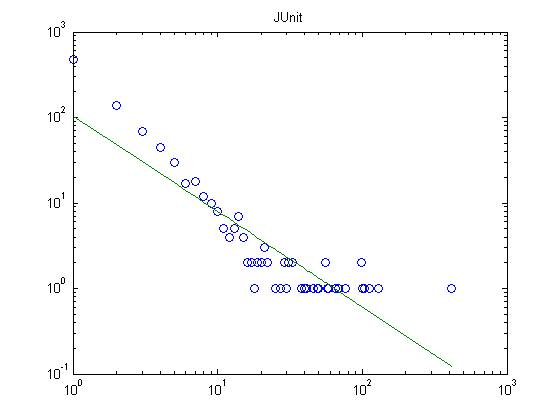
\includegraphics[scale=0.45]{images/marsold}
\end{figure}
For every project we analyzed, we saw clear linear trends at the initial segment of the
data, which is highly suggestive of the power law nature of the degree distribution.
Unfortunately, since the in-degree cannot be fractional, we begin seeing the tail
of this distribution getting flattened out to $y = 1$, which ends up heavily skewing
the exponent $\gamma$, as can be seen in figure \ref{fig:marsold}.

This ``skewing'' of the linear regression can be corrected by instead looking at the
cumulative density of the data \cite{CLASS}. Consider the probability density function
$p(k) = C k^{-\gamma}$ and let the random variable $K$ be such that $K = k$ is the
event that a random vertex has in-degree of $k$. We know that
$$P(K > k) = 1 - \sum_{i = 1}^k Ci^{-\gamma} = Ck^{1 - \gamma}.$$
The cumulative sum of the sample data is more stable because the low-frequency
tail will contribute negligibly to the cumulative sum if there are a lot of data already.
\begin{figure}[H]
\centering
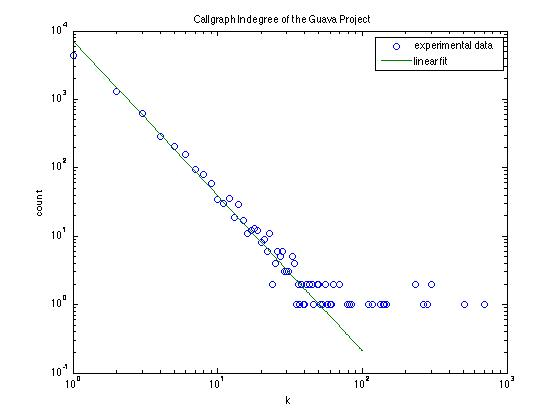
\includegraphics[scale=0.45]{images/guava}
\caption{Regression after fixing the fat-tail.\label{fig:guava}}
\end{figure}
Therefore, we found that if we compute the sample cumulative instead and get its
linear regression, we essentially remove all of the noise as can be see in figure
\ref{fig:guava}.
This is computed by the \g{cumulativeDistribution} subroutine within the code in
the appendix.
\begin{figure*}
\centering
\caption{Log-log degree distributions.\label{fig:deg}}
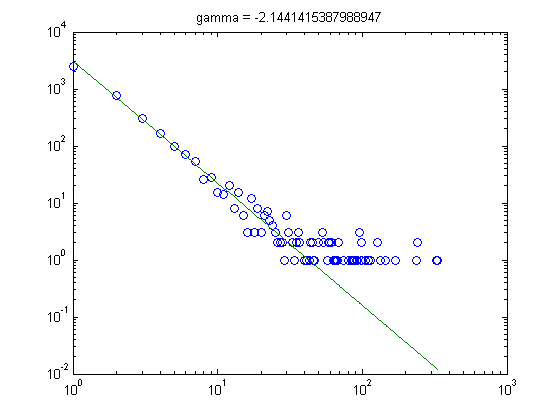
\includegraphics[scale=0.5]{images/antlr}
\includegraphics[scale=0.5]{images/JUNIT}

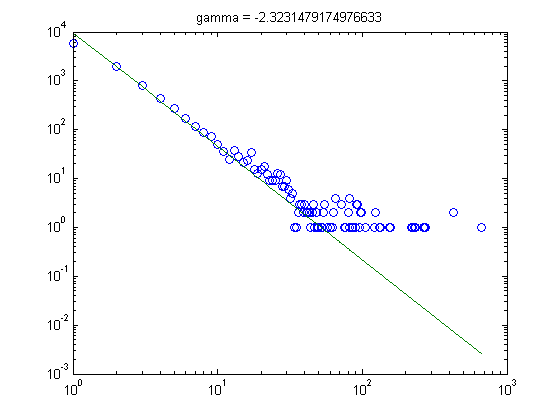
\includegraphics[scale=0.5]{images/logisim}
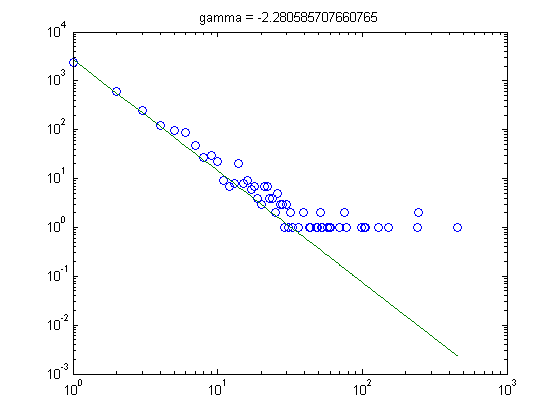
\includegraphics[scale=0.5]{images/MARS}

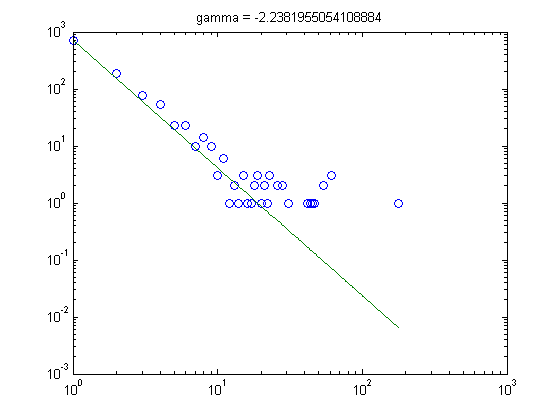
\includegraphics[scale=0.5]{images/webmagic}
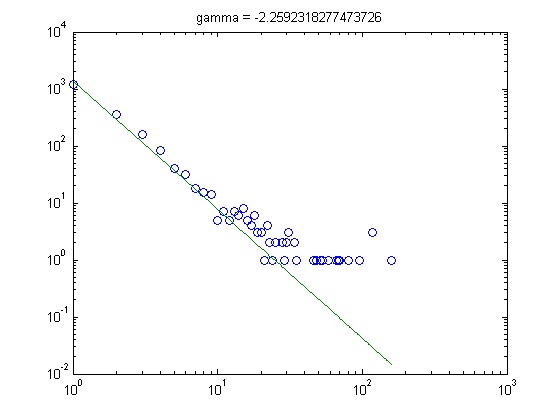
\includegraphics[scale=0.5]{images/xstream}
\end{figure*}
As we can see in figure \ref{fig:guava} and \ref{fig:deg}, the degree distributions of
all of the call-graphs we analyzed roughly follow power laws. In fact, we have a sample of
$\gamma$ of
% TODO Cite these projects
\begin{table}[H]
\centering
\begin{tabular}{|c|c|} \hline
Project & $\gamma$ \\ \hline
ANTLR & 2.1441 \\
Guava & 2.3121 \\
JUNIT & 2.1025 \\
Logisim & 2.3231 \\
MARS & 2.2806 \\
Webmagic & 2.2382 \\
Xstream & 2.2592 \\ \hline
\end{tabular}
\end{table}
\noindent which seems to be tightly packed around $2.2$. In fact, the sample mean is
$\bar \gamma = 2.2371$. Assuming that these observations are all independent
of one another, we can argue that the limiting distribution of these coefficients
is likely normal, so we can apply a statistical t-test with 6 degrees of freedom to find
that there is 95\% confidence that the population average of the coefficient $\gamma$
for all software projects is in the range $[2.159581, 2.314648]$. Therefore, we have
 statistically significant evidence to believe that on average
 $p(k) = O(k^{\bar \gamma})$ for some $\bar \gamma \in [2.159581, 2.314648]$.
\section{Conclusion}
By modeling the relationship of callee relationships within large java projects, we were
able to experimentally determine statistically significant evidence supporting
the claim that the density of the random event $K = k$\footnote{the event that a randomly
chosen vertex has in-degree $k$} roughly follows a power law on the order of around
$$p(k) = \frac{k^{-2.23}}{\zeta(2.23)}.$$ In addition, this scale-freeness property yields
the additional relationship that $k_{max}$, the degree of the most called function, is on the order of
$$k_{max} \sim O(\sqrt[1.23]{n})$$ where $n$ is the number of functions there are in the program.

Furthermore, this allows profilers to keep a quick estimate of the runtime complexity
of their large software on the order of $O(\sqrt[1.23]{n})$ where $n$ is the number of
lines\footnote{Best practice dictates that all functions should be less than $100$ lines
of code, so the number of functions is bounded above by an affine function of
the number of lines of code.} of code.
\subsection*{Limitations}
% TODO: someone do this part
% Also talk about directions for possible future work.

The main limitations of this method are the assumptions that need to be made in
order for the results to be valid.

As opposed to other methods which express runtime as a function relating input
length to an asymptotic number of steps, our method relates the number of steps
to the growth in \emph{lines of code} of a project. Further, our method can
only provide an approximation, whereas methods of the former type are exact
up to asymptotics.

In addition, our entire methodology is based on the assumption that the overall
runtime is approximately monotone with respect to the complexity of the
functions, meaning that the overall runtime only grows as the complexity of
each function grows. This is an approximation of real-life scenarios, since
it is not always true that increasing the size of a project increases its
runtime complexity.

\section{Related Works}
% TODO: someone do this part too

There has been a lot of research done on different kinds of runtime analysis as
well as scale-free networks. Scale-free networks have very unique characteristics
and have applications in a huge variety of topics. They can be used to analyze
static call graphs in programming as we have done as well as many other types
of networks. Examples include modeling protein networks to predict disease and
other ailments by observing the interactions between specific proteins.

%In the case of Google Guava, the distribution has coefficient $\gamma\approx
%2.7$, which suggests that it is within the realm of a scale-free network
%\cite{CLASS}.

\newpage
\printbibliography[title={References}]

% TODO appendix with source code

\end{singlespace}
\end{document}
